\documentclass[8pt,aspectratio=169]{beamer}
\usetheme{Madrid}
\usepackage{graphicx}
\usepackage{booktabs}
\usepackage{adjustbox}
\usepackage{multicol}
\usepackage{amsmath}
\usepackage{amssymb}
\usepackage{tikz}
\usepackage{hyperref}
\usepackage{algorithm}
\usepackage{algorithmic}
\usepackage{colortbl}
\usepackage{pgfplots}
\pgfplotsset{compat=1.18}

% TikZ libraries for comics, diagrams, stakeholder maps
\usetikzlibrary{arrows.meta,positioning,shapes.callouts,shapes.geometric,decorations.pathreplacing}

% Color definitions
\definecolor{mlblue}{RGB}{0,102,204}
\definecolor{mlpurple}{RGB}{51,51,178}
\definecolor{mllavender}{RGB}{173,173,224}
\definecolor{mllavender2}{RGB}{193,193,232}
\definecolor{mllavender3}{RGB}{204,204,235}
\definecolor{mllavender4}{RGB}{214,214,239}
\definecolor{mlorange}{RGB}{255, 127, 14}
\definecolor{mlgreen}{RGB}{44, 160, 44}
\definecolor{mlred}{RGB}{214, 39, 40}
\definecolor{mlgray}{RGB}{127, 127, 127}
\definecolor{lightgray}{RGB}{240, 240, 240}
\definecolor{midgray}{RGB}{180, 180, 180}

% NEW COLORS for mini-lecture
\definecolor{dfteal}{RGB}{0,128,128}
\definecolor{dfred}{RGB}{180,30,30}

% Backward compatibility
\colorlet{MLPurple}{mlpurple}
\colorlet{MLBlue}{mlblue}
\colorlet{MLOrange}{mlorange}
\colorlet{MLGreen}{mlgreen}
\colorlet{MLRed}{mlred}
\colorlet{MLLavender}{mllavender}
\colorlet{MLGray}{mlgray}

% Theme colors (exact Madrid settings)
\setbeamercolor{palette primary}{bg=mllavender3,fg=mlpurple}
\setbeamercolor{palette secondary}{bg=mllavender2,fg=mlpurple}
\setbeamercolor{palette tertiary}{bg=mllavender,fg=white}
\setbeamercolor{palette quaternary}{bg=mlpurple,fg=white}
\setbeamercolor{structure}{fg=mlpurple}
\setbeamercolor{section in toc}{fg=mlpurple}
\setbeamercolor{subsection in toc}{fg=mlblue}
\setbeamercolor{title}{fg=mlpurple}
\setbeamercolor{frametitle}{fg=mlpurple,bg=mllavender3}
\setbeamercolor{block title}{bg=mllavender2,fg=mlpurple}
\setbeamercolor{block body}{bg=mllavender4,fg=black}
\setbeamertemplate{navigation symbols}{}
\setbeamertemplate{itemize items}[circle]
\setbeamertemplate{enumerate items}[default]
\setbeamersize{text margin left=5mm,text margin right=5mm}

% Footer
\setbeamertemplate{footline}{
  \leavevmode%
  \hbox{%
    \begin{beamercolorbox}[wd=.333333\paperwidth,ht=2.25ex,dp=1ex,center]{author in head/foot}%
      \usebeamerfont{author in head/foot}Methods and Algorithms
    \end{beamercolorbox}%
    \begin{beamercolorbox}[wd=.333333\paperwidth,ht=2.25ex,dp=1ex,center]{title in head/foot}%
      \usebeamerfont{title in head/foot}MSc Data Science
    \end{beamercolorbox}%
    \begin{beamercolorbox}[wd=.333333\paperwidth,ht=2.25ex,dp=1ex,right]{date in head/foot}%
      \usebeamerfont{date in head/foot}\insertframenumber{} / \inserttotalframenumber\hspace*{2ex}
    \end{beamercolorbox}}%
  \vskip0pt%
}

\newcommand{\bottomnote}[1]{%
\vfill
\vspace{-2mm}
\textcolor{mllavender2}{\rule{\textwidth}{0.4pt}}
\vspace{1mm}
\footnotesize
\textbf{#1}
}

\newenvironment{compactlist}{%
  \begin{itemize}%
    \setlength{\itemsep}{2pt}%
    \setlength{\parskip}{0pt}%
    \setlength{\parsep}{0pt}%
}{%
  \end{itemize}%
}

\newcommand{\highlight}[1]{\textcolor{mlorange}{\textbf{#1}}}
\newcommand{\mathbold}[1]{\boldsymbol{#1}}

\title[Random Forests Mini-Lecture]{Random Forests}
\subtitle{A 10-Slide Mini-Lecture}
\author{Methods and Algorithms}
\institute{MSc Data Science}
\date{}

\begin{document}

%% ================================================================
%% SLIDE 1: WHY -- TikZ Comic (Dilemma)
%% ================================================================
\begin{frame}[t]{Why Would a Fraud Analyst Trust 500 Weak Detectors Over One Expert?}
\begin{columns}[T]
\column{0.55\textwidth}
\small
\textbf{The Dilemma}
\begin{compactlist}
\item \footnotesize A single decision tree overfits to training noise
\item \footnotesize High variance: different samples produce wildly different trees
\item \footnotesize Two trees can disagree completely on the same transaction
\item \footnotesize What if you let 500 imperfect trees vote?
\end{compactlist}
\vspace{2mm}
\begin{block}{Insight}
\footnotesize RF combines many weak learners --- variance drops without increasing bias.
\end{block}

\column{0.42\textwidth}
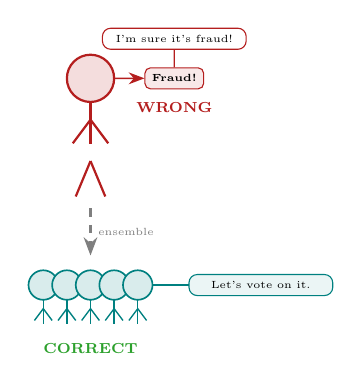
\begin{tikzpicture}[scale=0.75, every node/.style={transform shape}]
% Single tree figure -- wrong
\node[circle, draw=dfred, fill=dfred!15, minimum size=8mm, line width=0.8pt] (solo) at (0,3.5) {};
\draw[dfred, line width=0.8pt] (solo.south) -- ++(0,-0.7);
\draw[dfred, line width=0.8pt] (-0.3,2.4) -- (0,2.8) -- (0.3,2.4);
\draw[dfred, line width=0.8pt] (0,2.1) -- (-0.25,1.5);
\draw[dfred, line width=0.8pt] (0,2.1) -- (0.25,1.5);
% "Fraud!" sign
\node[rounded corners=2pt, draw=dfred, fill=dfred!10, font=\tiny\bfseries, right=5mm of solo] (sign) {Fraud!};
\draw[-{Stealth}, dfred, line width=0.6pt] (solo.east) -- (sign.west);
% Speech bubble
\node[rounded corners=3pt, draw=dfred, fill=white, font=\tiny, text width=2.2cm, align=center, above=3mm of sign] (bubble) {I'm sure it's fraud!};
\draw[dfred, line width=0.5pt] (bubble.south) -- (sign.north);
% Wrong mark
\node[font=\scriptsize\bfseries, text=dfred, below=1mm of sign] {WRONG};

% Crowd of 5 tree figures -- correct
\foreach \x/\lbl in {-0.8/1, -0.4/2, 0/3, 0.4/4, 0.8/5} {
  \node[circle, draw=dfteal, fill=dfteal!15, minimum size=5mm, line width=0.6pt] (t\lbl) at (\x,0) {};
  \draw[dfteal, line width=0.5pt] (t\lbl.south) -- ++(0,-0.4);
  \draw[dfteal, line width=0.5pt] (\x-0.15,-0.6) -- (\x,-0.4) -- (\x+0.15,-0.6);
}
% Thought bubble from crowd
\node[rounded corners=3pt, draw=dfteal, fill=dfteal!8, font=\tiny, text width=2.2cm, align=center, right=6mm of t5] (thought) {Let's vote on it.};
\draw[dfteal, line width=0.5pt] (thought.west) -- (t5.east);
% Correct mark
\node[font=\scriptsize\bfseries, text=mlgreen, below=6mm of t3] {CORRECT};

% Arrow from solo to crowd
\draw[-{Stealth}, mlgray, line width=0.8pt, dashed] (0,1.3) -- node[right, font=\tiny, text=mlgray]{ensemble} (0,0.5);
\end{tikzpicture}
\end{columns}
\bottomnote{Ensemble learning = combining imperfect models to produce reliable decisions}
\end{frame}

%% ================================================================
%% SLIDE 2: FEEL -- Reflection Prompt
%% ================================================================
\begin{frame}[t]{Polling the Room vs.\ Asking One Expert -- Which Do You Trust More?}
\begin{columns}[T]
\column{0.55\textwidth}
\small
\textbf{Think Before You Compute}

\footnotesize
Imagine asking one friend for a restaurant recommendation versus polling 20 friends. The single friend might have a strong bias (loves sushi, hates Italian). But 20 friends? Their biases cancel, and the consensus is more stable.
\begin{compactlist}
\item \footnotesize How many friends would you ask?
\item \footnotesize Did their individual biases cancel out?
\item \footnotesize Was the consensus more stable than any single opinion?
\end{compactlist}
\vspace{2mm}
\begin{exampleblock}{Reflection Prompt}
\footnotesize Think of a time you made a better decision by gathering multiple opinions.
\end{exampleblock}

\column{0.42\textwidth}
\vspace{8mm}
\fcolorbox{mlpurple}{mlpurple!10}{%
\parbox{0.9\columnwidth}{%
\footnotesize
\textcolor{mlpurple}{\textbf{Pause and reflect:}} when you last chose a restaurant by asking friends, you were bagging human opinions.%
}}
\end{columns}
\bottomnote{Bootstrap aggregating (bagging) formalizes this intuition: sample, train, average}
\end{frame}

%% ================================================================
%% SLIDE 3: WHAT -- Taxonomy Table
%% ================================================================
\begin{frame}[t]{What Makes a Random Forest Different from Bagging, Boosting, and a Single Tree?}
\begin{columns}[T]
\column{0.55\textwidth}
\small
\textbf{Taxonomy of Ensemble Methods}

\vspace{1mm}
\footnotesize
\begin{adjustbox}{max width=\columnwidth}
\begin{tabular}{lcccc}
\toprule
\textbf{Property} & \textbf{RF} & \textbf{Bagging} & \textbf{Boosting} & \textbf{Single Tree} \\
\midrule
Sampling & Bootstrap & Bootstrap & Sequential & All \\
\rowcolor{mllavender4}
Feature subset & $\sqrt{p}$ & All & All & All \\
Tree correlation & Low & High & Sequential & N/A \\
\rowcolor{mllavender4}
Bias & Low & Low & Low & Low \\
Variance & Low & Medium & Low & High \\
\rowcolor{mllavender4}
Parallel & Yes & Yes & No & N/A \\
\bottomrule
\end{tabular}
\end{adjustbox}
\vspace{2mm}
\begin{block}{Insight}
\footnotesize RF adds feature randomization \textbf{on top of} bagging to decorrelate trees.
\end{block}
\vspace{0.3em}
\scriptsize \textbf{Default split criterion:} $G(p) = 1 - \sum_{k=1}^{K} p_k^2$ \quad (Gini impurity)

\column{0.42\textwidth}
\vspace{2mm}
% Four colored summary boxes
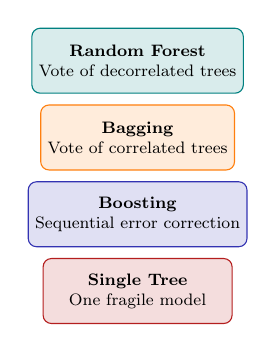
\begin{tikzpicture}[scale=0.75, every node/.style={transform shape}]
\node[rounded corners=3pt, draw=dfteal, fill=dfteal!15, minimum width=3.2cm,
      minimum height=1.1cm, font=\footnotesize, align=center, text=black] at (0,3.2)
      {\textbf{Random Forest}\\Vote of decorrelated trees};
\node[rounded corners=3pt, draw=mlorange, fill=mlorange!15, minimum width=3.2cm,
      minimum height=1.1cm, font=\footnotesize, align=center, text=black] at (0,1.9)
      {\textbf{Bagging}\\Vote of correlated trees};
\node[rounded corners=3pt, draw=mlpurple, fill=mlpurple!15, minimum width=3.2cm,
      minimum height=1.1cm, font=\footnotesize, align=center, text=black] at (0,0.6)
      {\textbf{Boosting}\\Sequential error correction};
\node[rounded corners=3pt, draw=dfred, fill=dfred!15, minimum width=3.2cm,
      minimum height=1.1cm, font=\footnotesize, align=center, text=black] at (0,-0.7)
      {\textbf{Single Tree}\\One fragile model};
\end{tikzpicture}
\end{columns}
\bottomnote{Breiman (2001) showed feature randomization is what makes RF variance reduction superior to plain bagging}
\end{frame}

%% ================================================================
%% SLIDE 4: CASE -- Step Diagram
%% ================================================================
\begin{frame}[t]{How Does a Single Transaction Navigate 500 Trees to a Fraud Verdict?}
\begin{columns}[T]
\column{0.55\textwidth}
\small
\textbf{One Transaction, 500 Votes}
\begin{compactlist}
\item \footnotesize Bootstrap sample 63.2\% of training data per tree
\item \footnotesize At each split, consider only $\sqrt{p}$ random features
\item \footnotesize Each tree votes: fraud or legit
\item \footnotesize Majority vote = final prediction
\item \footnotesize OOB samples validate without a held-out test set
\end{compactlist}
\vspace{2mm}
\begin{block}{Insight}
\footnotesize Each tree sees different data AND different features -- this double randomness is the source of RF's power.
\end{block}

\column{0.42\textwidth}
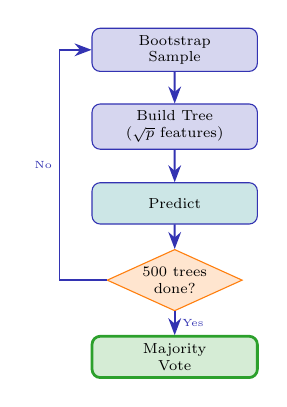
\begin{tikzpicture}[scale=0.75, every node/.style={transform shape},
  stepbox/.style={rounded corners=3pt, draw=mlpurple,
               minimum width=2.8cm, minimum height=0.7cm,
               font=\scriptsize, align=center},
  arr/.style={-{Stealth}, line width=0.7pt, mlpurple}]
\node[stepbox, fill=mllavender4] (s1) at (0,4.5) {Bootstrap\\Sample};
\node[stepbox, fill=mllavender4] (s2) at (0,3.2) {Build Tree\\($\sqrt{p}$ features)};
\node[stepbox, fill=dfteal!20] (s3) at (0,1.9) {Predict};
\node[diamond, draw=mlorange, fill=mlorange!20, aspect=2.2,
      font=\scriptsize, align=center, inner sep=1pt] (s4) at (0,0.6) {500 trees\\done?};
\node[stepbox, fill=mlgreen!20, draw=mlgreen, line width=1pt] (s5) at (0,-0.7) {Majority\\Vote};
\draw[arr] (s1) -- (s2);
\draw[arr] (s2) -- (s3);
\draw[arr] (s3) -- (s4);
\draw[arr] (s4) -- node[right, font=\tiny]{Yes} (s5);
\draw[arr] (s4.west) -- ++(-0.8,0) |- node[left, font=\tiny, pos=0.25]{No} (s1.west);
\end{tikzpicture}
\end{columns}
\bottomnote{63.2\% = $1 - (1-1/n)^{n} \to 1 - 1/e$ for large $n$}
\end{frame}

%% ================================================================
%% SLIDE 5: HOW -- Decorrelation Trick
%% ================================================================
\begin{frame}[t]{How Does Feature Randomization Kill the Correlation Between Trees?}
\begin{columns}[T]
\column{0.55\textwidth}
\small
\textbf{The Decorrelation Trick}
\begin{compactlist}
\item \footnotesize Bagging alone: if one feature dominates, all trees split on it --- correlated --- slow variance reduction
\item \footnotesize RF fix: restrict each split to $\sqrt{p}$ random features --- different trees use different features --- $\rho$ drops
\item \footnotesize $\text{Var}(\bar{f}) = \rho\sigma^{2} + \dfrac{1-\rho}{B}\sigma^{2}$
\end{compactlist}
\vspace{2mm}
\begin{block}{Insight}
\footnotesize Reducing $\rho$ is more powerful than increasing $B$.
\end{block}

\column{0.42\textwidth}
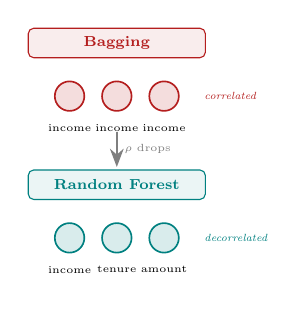
\begin{tikzpicture}[scale=0.75, every node/.style={transform shape}]
% Bagging box
\node[rounded corners=2pt, draw=dfred, fill=dfred!8,
      minimum width=3cm, minimum height=0.5cm, font=\scriptsize\bfseries]
      (blbl) at (0,4.2) {\textcolor{dfred}{Bagging}};
\node[circle, draw=dfred, fill=dfred!15, minimum size=5mm, font=\tiny, line width=0.6pt]
      (b1) at (-0.8,3.3) {};
\node[circle, draw=dfred, fill=dfred!15, minimum size=5mm, font=\tiny, line width=0.6pt]
      (b2) at (0,3.3) {};
\node[circle, draw=dfred, fill=dfred!15, minimum size=5mm, font=\tiny, line width=0.6pt]
      (b3) at (0.8,3.3) {};
\node[font=\tiny, below=1mm of b1] {income};
\node[font=\tiny, below=1mm of b2] {income};
\node[font=\tiny, below=1mm of b3] {income};
\node[font=\tiny\itshape, text=dfred, right=3mm of b3] {correlated};

% RF box
\node[rounded corners=2pt, draw=dfteal, fill=dfteal!8,
      minimum width=3cm, minimum height=0.5cm, font=\scriptsize\bfseries]
      (rlbl) at (0,1.8) {\textcolor{dfteal}{Random Forest}};
\node[circle, draw=dfteal, fill=dfteal!15, minimum size=5mm, font=\tiny, line width=0.6pt]
      (r1) at (-0.8,0.9) {};
\node[circle, draw=dfteal, fill=dfteal!15, minimum size=5mm, font=\tiny, line width=0.6pt]
      (r2) at (0,0.9) {};
\node[circle, draw=dfteal, fill=dfteal!15, minimum size=5mm, font=\tiny, line width=0.6pt]
      (r3) at (0.8,0.9) {};
\node[font=\tiny, below=1mm of r1] {income};
\node[font=\tiny, below=1mm of r2] {tenure};
\node[font=\tiny, below=1mm of r3] {amount};
\node[font=\tiny\itshape, text=dfteal, right=3mm of r3] {decorrelated};

% Arrow between
\draw[-{Stealth}, mlgray, line width=0.8pt] (0,2.7) -- node[right, font=\tiny, text=mlgray]{$\rho$ drops} (0,2.1);
\end{tikzpicture}
\end{columns}
\bottomnote{$\text{Var}(\text{RF}) = \rho\sigma^{2} + (1-\rho)\sigma^{2}/B$ -- the first term is the irreducible correlation floor}
\end{frame}

%% ================================================================
%% SLIDE 6: RISK -- Three Failure Modes
%% ================================================================
\begin{frame}[t]{What Happens When the Forest Memorizes Noise Instead of Signal?}
\begin{columns}[T]
\column{0.55\textwidth}
\small
\textbf{Three Ways RF Can Still Fail}
\begin{compactlist}
\item \footnotesize \textbf{Overfitting to noise:} too many deep trees on small data
\item \footnotesize \textbf{Feature leakage:} a feature that encodes the label
\item \footnotesize \textbf{Class imbalance:} RF votes majority --- rare class outvoted
\end{compactlist}
\vspace{2mm}
\begin{block}{Insight}
\footnotesize Class imbalance is the \#1 failure mode in fraud detection -- always check class distribution.
\end{block}

\column{0.42\textwidth}
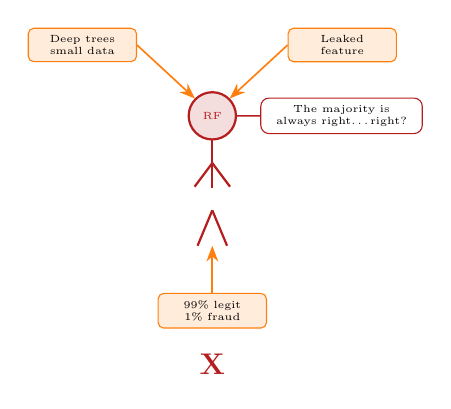
\begin{tikzpicture}[scale=0.75, every node/.style={transform shape}]
% RF stick figure -- frustrated
\node[circle, draw=dfred, fill=dfred!15, minimum size=8mm, line width=0.8pt] (rf) at (0,2) {};
\node[font=\tiny, text=dfred] at (0,2) {RF};
\draw[dfred, line width=0.8pt] (rf.south) -- ++(0,-0.8);
\draw[dfred, line width=0.8pt] (-0.3,0.8) -- (0,1.2) -- (0.3,0.8);
\draw[dfred, line width=0.8pt] (0,0.4) -- (-0.25,-0.2);
\draw[dfred, line width=0.8pt] (0,0.4) -- (0.25,-0.2);

% Danger sign 1: deep trees on small data
\node[rounded corners=2pt, draw=mlorange, fill=mlorange!15,
      font=\tiny, align=center, text width=1.6cm] (d1) at (-2.2,3.2) {Deep trees\\small data};
% Danger sign 2: leaked feature
\node[rounded corners=2pt, draw=mlorange, fill=mlorange!15,
      font=\tiny, align=center, text width=1.6cm] (d2) at (2.2,3.2) {Leaked\\feature};
% Danger sign 3: imbalanced pie
\node[rounded corners=2pt, draw=mlorange, fill=mlorange!15,
      font=\tiny, align=center, text width=1.6cm] (d3) at (0,-1.3) {99\% legit\\1\% fraud};

\draw[-{Stealth}, mlorange, line width=0.6pt] (d1.east) -- (rf.north west);
\draw[-{Stealth}, mlorange, line width=0.6pt] (d2.west) -- (rf.north east);
\draw[-{Stealth}, mlorange, line width=0.6pt] (d3.north) -- (0,-0.2);

% Speech bubble
\node[rounded corners=3pt, draw=dfred, fill=white, font=\tiny,
      text width=2.5cm, align=center, right=4mm of rf] (spk)
      {The majority is always right\ldots right?};
\draw[dfred, line width=0.5pt] (spk.west) -- (rf.east);

% Large red X
\node[font=\Large\bfseries, text=dfred] at (0,-2.2) {X};
\end{tikzpicture}
\end{columns}
\bottomnote{Solutions: max\_depth, min\_samples\_leaf, class\_weight='balanced', SMOTE for resampling}
\end{frame}

%% ================================================================
%% SLIDE 7: WHERE -- Industry Default + Chart
%% ================================================================
\begin{frame}[t]{Why Do So Many Fraud Teams Reach for Random Forests First?}
\begin{columns}[T]
\column{0.55\textwidth}
\small
\textbf{RF as the Industry Default}
\begin{compactlist}
\item \footnotesize Ensemble voting aggregates weak signals
\item \footnotesize Feature importance reveals which attributes matter
\item \footnotesize OOB error = free cross-validation
\item \footnotesize Scales to millions with parallel training
\end{compactlist}
\vspace{2mm}
\begin{block}{Insight}
\footnotesize RF popularity = simplest reasonable solution that works out of the box.
\end{block}

\column{0.42\textwidth}
\vspace{2mm}
\includegraphics[width=\textwidth]{05_ensemble_voting/chart.pdf}
\end{columns}
\bottomnote{Kaggle surveys rank RF/gradient boosting as top methods for tabular data}
\end{frame}

%% ================================================================
%% SLIDE 8: IMPACT -- Stakeholder Map
%% ================================================================
\begin{frame}[t]{Who Wins and Who Loses When Trees Replace Rules?}
\begin{columns}[T]
\column{0.55\textwidth}
\small
\textbf{Stakeholder Analysis}
\begin{compactlist}
\item \footnotesize \textbf{Winners:} Fraud analysts (better detection), Risk managers (feature importance for audit), Data engineers (parallel, easy deploy)
\item \footnotesize \textbf{Losers:} Compliance officers (less interpretable than logistic regression), Customers flagged by opaque ensemble
\end{compactlist}
\vspace{2mm}
\begin{block}{Insight}
\footnotesize RF shifts fraud detection from human-crafted rules to data-driven patterns.
\end{block}

\column{0.42\textwidth}
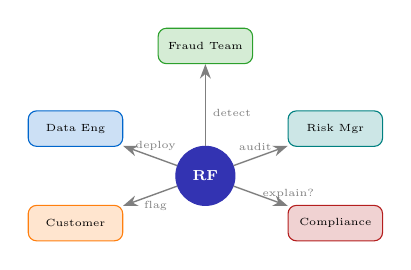
\begin{tikzpicture}[scale=0.75, every node/.style={transform shape},
  arr/.style={-{Stealth}, line width=0.5pt, mlgray}]
% Center RF node
\node[circle, draw=mlpurple, fill=mlpurple, minimum size=1cm,
      font=\scriptsize\bfseries, text=white] (rf) at (0,0) {RF};
% Stakeholders
\node[rounded corners=3pt, draw=mlgreen, fill=mlgreen!20,
      minimum width=1.6cm, minimum height=0.6cm,
      font=\tiny, align=center, text=black] (fraud) at (0,2.2) {Fraud Team};
\node[rounded corners=3pt, draw=dfteal, fill=dfteal!20,
      minimum width=1.6cm, minimum height=0.6cm,
      font=\tiny, align=center, text=black] (risk) at (2.2,0.8) {Risk Mgr};
\node[rounded corners=3pt, draw=dfred, fill=dfred!20,
      minimum width=1.6cm, minimum height=0.6cm,
      font=\tiny, align=center, text=black] (comp) at (2.2,-0.8) {Compliance};
\node[rounded corners=3pt, draw=mlorange, fill=mlorange!20,
      minimum width=1.6cm, minimum height=0.6cm,
      font=\tiny, align=center, text=black] (cust) at (-2.2,-0.8) {Customer};
\node[rounded corners=3pt, draw=mlblue, fill=mlblue!20,
      minimum width=1.6cm, minimum height=0.6cm,
      font=\tiny, align=center, text=black] (eng) at (-2.2,0.8) {Data Eng};
% Arrows with labels
\draw[arr] (rf) -- node[right, font=\tiny, pos=0.4]{detect} (fraud);
\draw[arr] (rf) -- node[above, font=\tiny, pos=0.4]{audit} (risk);
\draw[arr] (rf) -- node[right, font=\tiny, pos=0.4]{explain?} (comp);
\draw[arr] (rf) -- node[below, font=\tiny, pos=0.4]{flag} (cust);
\draw[arr] (rf) -- node[above, font=\tiny, pos=0.4]{deploy} (eng);
\end{tikzpicture}
\end{columns}
\bottomnote{ECOA and GDPR require adverse action explanations -- SHAP values bridge the gap}
\end{frame}

%% ================================================================
%% SLIDE 9: SO WHAT -- Decision Framework
%% ================================================================
\begin{frame}[t]{When Should You Reach for Random Forests -- and When Should You Not?}
\begin{columns}[T]
\column{0.55\textwidth}
\small
\textbf{The Decision Framework}
\begin{enumerate}
\item \footnotesize \textbf{Is your data tabular?} If images/text $\to$ deep learning.
\item \footnotesize \textbf{Do you need probability calibration?} RF probabilities often poorly calibrated $\to$ Platt scaling.
\item \footnotesize \textbf{Must the model be fully interpretable?} If yes $\to$ logistic regression or single tree.
\end{enumerate}
\vspace{2mm}
\begin{block}{Insight}
\footnotesize No Free Lunch: RF excels on tabular, non-linear, feature-rich data.
\end{block}

\column{0.42\textwidth}
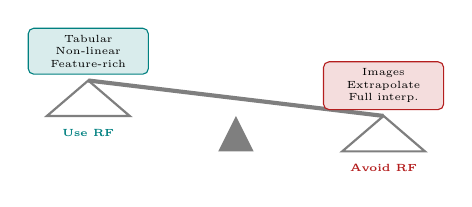
\begin{tikzpicture}[scale=0.75, every node/.style={transform shape}]
% Fulcrum
\fill[mlgray] (0,-0.3) -- (-0.3,-0.9) -- (0.3,-0.9) -- cycle;
% Beam (tilted: left heavier)
\draw[mlgray, line width=1.5pt] (-2.5,0.3) -- (2.5,-0.3);
% Left pan (heavier, lower)
\coordinate (ltop) at (-2.5,0.3);
\coordinate (lbot) at (-2.5,-0.3);
\draw[mlgray, line width=0.8pt] (ltop) -- (-3.2,-0.3) -- (-1.8,-0.3) -- cycle;
\node[rounded corners=2pt, fill=dfteal!15, draw=dfteal,
      font=\tiny, align=center, text width=1.8cm, above=1mm of ltop] (lpan)
      {Tabular\\Non-linear\\Feature-rich};
\node[font=\tiny\bfseries, text=dfteal, below=1mm of lbot] {Use RF};

% Right pan (lighter, higher)
\coordinate (rtop) at (2.5,-0.3);
\coordinate (rbot) at (2.5,-0.9);
\draw[mlgray, line width=0.8pt] (rtop) -- (1.8,-0.9) -- (3.2,-0.9) -- cycle;
\node[rounded corners=2pt, fill=dfred!15, draw=dfred,
      font=\tiny, align=center, text width=1.8cm, above=1mm of rtop] (rpan)
      {Images\\Extrapolate\\Full interp.};
\node[font=\tiny\bfseries, text=dfred, below=1mm of rbot] {Avoid RF};
\end{tikzpicture}
\end{columns}
\bottomnote{When in doubt: start with RF as baseline, then try XGBoost/LightGBM for marginal improvement}
\end{frame}

%% ================================================================
%% SLIDE 10: ACT -- Diagnostic Exercise
%% ================================================================
\begin{frame}[t]{Can You Diagnose This Fraud Detection Model?}
\begin{columns}[T]
\column{0.55\textwidth}
\small
\textbf{The Scenario}

\footnotesize
A payment processor runs RF with 1000 trees. Features: amount, time, merchant category, distance from home, device fingerprint. Flags 2\% as fraud; actual fraud rate is 0.1\%.
\begin{compactlist}
\item \footnotesize Calculate the expected false positive rate
\item \footnotesize Which feature likely ranks highest in importance?
\item \footnotesize Model misses 40\% of fraud -- what would you change?
\item \footnotesize Is the OOB error reliable here?
\end{compactlist}
\vspace{2mm}
\begin{exampleblock}{Deliverable}
\footnotesize Fill in the table on the right.
\end{exampleblock}

\column{0.42\textwidth}
\centering
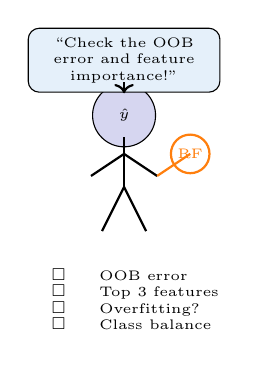
\begin{tikzpicture}[scale=0.7]
% Detective figure
\node[circle,draw,fill=mlpurple!20,minimum size=0.8cm,font=\tiny] (head) at (0,2.5) {$\hat{y}$};
\draw[thick] (0,2.1) -- (0,1.2);
\draw[thick] (0,1.8) -- (-0.6,1.4);
\draw[thick] (0,1.8) -- (0.6,1.4);
\draw[thick] (0,1.2) -- (-0.4,0.4);
\draw[thick] (0,1.2) -- (0.4,0.4);
% Magnifying glass
\draw[thick,mlorange] (0.6,1.4) -- (1.2,1.8);
\draw[thick,mlorange] (1.2,1.8) circle (0.35);
\node[font=\tiny,mlorange] at (1.2,1.8) {RF};
% Speech bubble
\node[draw,rounded corners,fill=mlblue!10,font=\tiny,text width=2.2cm,align=center] at (0,3.5) {``Check the OOB error and feature importance!''};
% Arrow from bubble to head
\draw[->,thick] (0,3.1) -- (0,2.9);
% Checklist
\node[font=\tiny,anchor=north west] at (-1.5,-0.1) {
\begin{tabular}{@{}ll@{}}
$\square$ & OOB error \\
$\square$ & Top 3 features \\
$\square$ & Overfitting? \\
$\square$ & Class balance \\
\end{tabular}
};
\end{tikzpicture}
\end{columns}
\bottomnote{Hint: with 0.1\% fraud rate and 2\% flag rate, most flags are false positives}
\end{frame}

\end{document}
